
\section{Soundness of our proof system}

In this section we will prove that the proof system presented in section \ref{sect:proofSystem} is sound. We give the usual meaning to the Hoare triples (Sect \ref{sect:HLmeans}), we prove soundness of of Hoare triples (Sect \ref{sect:prove:triples:sound}), we show how execution starting from some external state can be summarised into purely external execution and terminating execution of public methods (Sect \ref{sect:termExecs}), and use these decompositions and a well-founded ordering to prove soundness of our quadruples  (Sect \ref{sect:prove:sound:quadruples}), and then prove soundness of the overall system  (Sect \ref{sect:prove:triples:overall}). 



We start by requiring  that the supporting proof system for assertions, and for encapsulation are sound.
\begin{axiom}
\label{lemma:axiom:enc:assert}
We assume a judgment of the form $M \vdash A$,  a judgment of the form $M \vdash \encaps{A}$, which have the property that
\begin{center}
$M \vdash A $ \ \ \ \ implies \ \ \ \ $M \vDash A$.\\
 $M \vdash \encaps{A} $ \ \ \ \ implies \ \ \ \ $M \vDash \encaps{A}$.
 \end{center}
\end{axiom}

%%%%%%%%%%%%%%%%%%%%%%%%%%%%%%%%%%%%%%%%%%%%%%%%%%%

\subsection{Semantics of Hoare triples and quadruples}
\label{sect:HLmeans}

We  define the {\emph {meaning}} of  our Hoare triples, $\triple {A} {stmt} {A'}$,  in the usual way, \ie that execution of $stmt$ in a state that satisfies $A$ leads to a state which satisfies $A'$.  
In addition to that, Hoare quadruples, $\quadruple {A} {stmt} {A'} {A''}$, promise that any external future states scoped by $\sigma$ will satisfy $A''$.

 
\begin{definition}[Semantics of Hoare tuples]
\label{def:hoare:sem}
 
For modules $M$, and assertions $A$, $A'$   we define:
%  the semantics of Hoare-triples,   $M\ \models\  \{\, A \,  \}\ stmt\  \{\, A' \, \}$ as follows:
\begin{itemize}
\item
\label{def:hoare:sem:three}
$M\ \models\  \{\, A \,  \}\ stmt\  \{\, A' \, \}$ \\
if\
 for   all $\Mtwo$, for all $\sigma$, $\sigma'$ such that {$\arising \sigma {\Mtwo\cdot M}$}\\
$\strut ~ ~ ~ ~ [ \ \ M,\sigma \ \models \ A \ \wedge\  
 \sigma.cont = stmt  \ \wedge\     \leadstoBoundedStarFin {\Mtwo\cdot M}  {\sigma}  {\sigma'}    \ \ \Longrightarrow\ \ M,\sigma' \ \models \ A'\ \ ]$
 
 \item
 \label{def:hoare:sem:four}
 $M\ \models\ \quadruple {A} {stmt} {A'} {A''}$ \\
if\\
$M\ \models\  \triple  {A} {stmt} {A'} $, and\\
  for   all $\Mtwo$, for all $\sigma$, $\sigma''$ such that {$\arising \sigma {\Mtwo\cdot M}$}\\
$\strut ~ ~ ~ ~ [ \ \ M,\sigma \ \models \ A \ \wedge\  
 \sigma.cont = stmt  \ \wedge\     \leadstoBoundedStar  {\Mtwo\cdot M}  {\sigma}  {\sigma''}  % \ \wedge \   M,\sigma \ \models \ \ 
 \ \ \Longrightarrow\ \ M,\sigma'' \ \models \ \extThis  \rightarrow A''\ \ ]$

\end{itemize}
\end{definition}

%%%%%%%%%%%%%%%%%%%%%%%%%%%%%%%%%%%%%%%%%%%%%%%%%%%

\subsection{Soundness of the Hoare Triples Logic}
\label{sect:prove:triples:sound}
We first prove soundness of the inference system for triples $M \vdash  \triple A {stmt} {A'} $:

\sdN{
\begin{auxLemma}
\label{l:no:call}
For any module $M$, assertions $A$, $A'$ and $A''$, and statement $stmt$ which does not contain any method call:
 \\
$\strut \hspace{2cm} M\ \models\ \triple {A} {stmt}   {A'} \ \ \Longrightarrow\ \  M\ \models\ \quadruple {A} {stmt}   {A'} {A''}$
\end{auxLemma}
}


\begin{theorem}
\label{l:triples:sound}
For module  $M$ % and $\Mtwo$, 
such that  $\vdash M$, and for any assertions $A$,  $A'$, $A''$ and statement  $stmt$:
\sdN{
\begin{center}
$M\ \vdash\  \triple A {stmt} {A'}$ \ \ \ \ $\Longrightarrow$ \ \ \ \ $M\ \models\   \quadruple A {stmt} {A'} {A''}$
\end{center}
}
\end{theorem}
 

\noindent
\vspace{.2cm}
%  {\textbf{Proof Sketch}} 
%\noindent
%Take any $M$, $\Mtwo$, $A$, $A'$, $A''$, and $stmt$.
%Assume that \\
%$\strut \ \ \hspace{2.3cm} \ \ (1) \ \ M\ \vdash\  \triple A {stmt} {A'}$ 
%\\
%We want to show  that\\
% $\strut \ \ \hspace{2.3cm} \ \ (\alpha) \  \ M\ \models\   \quadruple A {stmt} {A'} {A''}$
% \\ 
The proof goes by case analysis over the rule applied to obtain $M \vdash \{ A \}\ stmt \  \{ A' \} $:

\begin{description} 

\item[${\sc{extend}}$] 

By soundness of the underlying Hoare logic, we obtain that  $M\ \models\ \triple {A} {stmt}   {A'}$. Moreover, 
by the assumption of {\sc{extend}}, $stmt$ does not contain any method call. Rest follows by lemma \ref{l:no:call}.

\item[${\sc{types-1}}$] 

Follows from type system, the assumption of {\sc{types-1}} and lemma \ref{l:no:call}.

\item[${\sc{prot-1}}$]  
Therefore, $A \txteq ....$ and $A' \txteq ....$  and $stmt \txteq y=y'.f$ .... TODO: write rest of proof ...
Rest follows by lemma \ref{l:no:call}.
\item[${\sc{prot-2}}$] ... Rest follows by lemma \ref{l:no:call}.

\item[${\sc{prot-3}}$] ... Rest follows by lemma \ref{l:no:call}.

\item[${\sc{prot-4}}$] ... Rest follows by lemma \ref{l:no:call}.

\end{description}
\noindent
\vspace{.1cm}
  {\textbf{End Proof Sketch}} 

 
\subsection{Summarized  execution} 

\label{sect:termExecs}

\sdN{
\begin{definition}
The shorthand $M, \sigma \models \extThis$  expresses that $M, \sigma \models \external{\prg{this}}$, and
$M, \sigma \models \pubMeth$ expresses that the currently executing method is public.\footnote{Need to expand the state accordingly}
\end{definition}
}


\label{sect:termExecs}
% In order to prove the soundness of our proof rules (\ie that $M \models  \{\, A \,  \}\ stmt\  \{\, A' \, \}$ implies that $M \vdash  \{\, A \,  \}\ stmt\  \{\, A' \, \}$,
We also need some auxiliary properties of the operational semantics.
 
Lemma \ref{lemma:encl:tem} guarantees that any state reachable from a state with a terminating execution has itself a terminating execution, and that this execution is enclosed in the original one:
 
 \begin{auxLemma}[Enclosed Terminating Executions]\footnote{TODO find better name for the aux lemma}
 \label{lemma:encl:tem}
 For any modules $\Mtwo$,   and states $\sigma$, $\sigma'$, $\sigma_1$:
\begin{itemize}
\item
$  \leadstoBoundedStarFin {\Mtwo}  {\sigma}  {\sigma'} \  \wedge \  \leadstoBoundedStar  {\Mtwo}  {\sigma}  {\sigma_1} 
% $\\ $
\ \ \  \Longrightarrow\ \ \  % $\\ $  
 \exists \sigma_2.[\ \ \leadstoBoundedStarFin {\Mtwo} {\sigma_1}  {\sigma_2}  
\ \wedge\ 
\leadstoBoundedStarThree  {\Mtwo}  {\sigma_2}  {\sigma}   {\sigma'} \ \ ]$
\end{itemize}

\end{auxLemma} 
 
Lemma \ref{lemma:subexp} makes the usual guarantee about terminating execution of statement sequences.
  
\begin{auxLemma}[Execution of sequences]
\label{lemma:subexp}
For any modules $\Mtwo$, statements $s_1$, $s_2$, and states $\sigma$, $\sigma'$, $\sigma'''$:
\begin{itemize}
\item
$ \sigma.\texttt{cont} = s_1; s_2 \ \ \wedge\ \  \leadstoBoundedStarFin {\Mtwo}  {\sigma}  {\sigma'}\ \ 
\wedge \ \
\leadstoBoundedStar {\Mtwo}  {\sigma}  {\sigma''}\
$\\
$  \Longrightarrow$\\
$   \exists \sigma''.[\ \ \ \ \   \leadstoBoundedStarFin {\Mtwo} {\sigma[\texttt{cont}\mapsto s_1]}  {\sigma''}  
\ \wedge\ 
\leadstoBoundedStarFin {\Mtwo} {\sigma''[\texttt{cont}\mapsto s_2]}   {\sigma'} \  \wedge$
\\
$\strut \hspace{1.2cm}  [ \ \ \leadstoBoundedStar {\Mtwo} {\sigma[\texttt{cont}\mapsto s_1]}   {\sigma''}\ \vee \ \leadstoBoundedStar {\Mtwo}  {\sigma''[\texttt{cont}\mapsto s_2]}   {\sigma'''}\ ]\ \ \ \ \ \ \ \  \ ] $
\end{itemize}
\end{auxLemma}
 

Lemma \ref{lemma:external_breakdown} says that a terminating execution,  $ \leadstoBoundedStarFin {\Mtwo}  {\sigma}  {\sigma'}$ starting in an external state  consists of a sequence of  external states interleaved with terminating executions in internal states. 
It %of Auxialiry lemma \ref{lemma:external_breakdown} 
is illustrated through an example in Fig. \ref{fig:summaries}.
We fist define some further notations for execution:

\begin{definition}
For any module $M$  where $M$ is the internal module, external modules $\Mtwo$, and states $\sigma\bd$,  $\sigma$ and $\sigma'$, we define:

\begin{itemize}
\item
 ${\leadstoBoundedThreeStarExt {\Mtwo\cdot M} {\sigma\bd}  {\sigma}  {\sigma'}}$ \ \ \ \ \ $\triangleq$ \ \ 
$\begin{cases}
\exists n, \sigma_1, ... \sigma_n,\,  \mbox{s.t}\\
\strut \ \ \ \  \sigma = \sigma_1 \ \ \wedge\ \ \ \sigma' = \sigma_n \ \ \wedge \\
\strut \ \ \ \ \forall i\in [1..n).\ [ \ M, \sigma_i \models \extThis \ \wedge\  \leadstoBoundedThree {\Mtwo\cdot M} {\sigma_i}  {\sigma\bd}   
{\sigma_{i+1}}  \ ] \ \ \wedge \\
\strut \ \ \ \  M, \sigma'  \models  \extThis
% \\ \strut \ \ \ \  M, \sigma' \models \internal {\prg{this}} 
\end{cases}
$
% \sigma\bd not needed
%\item
%$\leadstoBoundedThreePub {\Mtwo\cdot M} {\sigma\bd}  {\sigma}  {\sigma'}$  \ \ if \ \ 
%$\begin{cases}
%\exists  \sigma_1, \sigma_2,\,  \mbox{s.t}\\
%\strut \ \ \ \  M, \sigma  \models \extThis \ \wedge \  \leadstoBoundedThree {\Mtwo\cdot M} {\sigma}  {\sigma\bd}   
%{\sigma_{1}} \\ 
%\strut \ \ \ \ \ M, \sigma_1 \models \pubMeth \ \wedge\  \leadstoBoundedStarFin {\Mtwo\cdot M} {\sigma_1}  {\sigma_2}    \ \ \wedge \\
%\strut \ \ \ \   \leadstoBoundedThree {\Mtwo\cdot M} {\sigma_2}   {\sigma\bd}  {\sigma'} 
%\end{cases}
%$
\item
${\WithPub {\Mtwo\cdot M}    {\sigma}  {\sigma'} {\sigma_1}}$ \  \ \ \ \  \ \ \ \ \ \ \ \ $\triangleq$ \ \ 
$\begin{cases}
\exists   \sigma_1',\,  \mbox{s.t}\\
\strut \ \ \ \  M, \sigma  \models \extThis \ \wedge \  \leadstoBoundedThree  {\Mtwo\cdot M} {\sigma} {\sigma}  {\sigma_{1}} \\ 
\strut \ \ \ \ \ M, \sigma_1 \models \pubMeth \ \wedge\  \leadstoBoundedStarFin {\Mtwo\cdot M} {\sigma_1}  {\sigma_1'}    \ \ \wedge \\
\strut \ \ \ \   \leadstoBounded  {\Mtwo\cdot M} {\sigma_1'}      {\sigma'} 
\end{cases}
$
\item
$\WithExtPub {\Mtwo\cdot M} {\sigma\bd}  {\sigma}  {\sigma'} {\epsilon} \ \ $   \ \  $\triangleq$ \ \ 
$\leadstoBoundedThreeStarExt {\Mtwo\cdot M} {\sigma\bd}  {\sigma}  {\sigma''}$
\item
$\WithExtPub {\Mtwo\cdot M} {\sigma\bd}  {\sigma}  {\sigma'} {\sigma_1...\sigma_n}$   \ \  $\triangleq$ \ \ 
$\exists \sigma'',\sigma'''.[\   {\leadstoBoundedThreeStarExt {\Mtwo\cdot M} {\sigma\bd}  {\sigma}  {\sigma''}}\ \wedge\ 
{\WithPub {\Mtwo\cdot M}    {\sigma''}  {\sigma'''} {\sigma_1}} \ \wedge$\\   
$\strut \hspace{8.2cm} {\WithExtPub {\Mtwo\cdot M} {\sigma\bd}  {\sigma'''}  {\sigma'} {\sigma_2...\sigma_n} }  \ ]$
%$\begin{cases}
%\strut \ \ \ \  \leadstoBoundedThreeStarExt  {\Mtwo\cdot M} {\sigma\bd}  {\sigma}  {\sigma'}\\
%\strut \ \ \ \   \ \mbox{or} \\
%\strut \ \ \ \  \exists \sigma_1, \sigma_2.[\  \\
%\strut \ \ \ \  \ \ \ \   \ \ \ \   \leadstoBoundedThreeStarExt  {\Mtwo\cdot M} {\sigma\bd}  {\sigma}  {\sigma_1} \ \wedge \ 
%\leadstoBoundedPub {\Mtwo\cdot M}  {\sigma_1}  {\sigma_2}\ \wedge \\ 
%\strut \ \ \ \  \ \ \ \   \ \ \ \  \leadstoBoundedThreeExtPub {\Mtwo\cdot M} {\sigma\bd}  {\sigma_1}  {\sigma_2}\  \ ]
%\end{cases}
%$
\item
$\leadstoBoundedExtPub {\Mtwo\cdot M}    {\sigma}  {\sigma'} $  \ \ \ \ \   \ \ \  \ \ \ \   \ \ \ \ $\triangleq$  \ \ 
$\strut \ \ \ \  \exists n\in \mathbb{N}. \exists \sigma_1,...\sigma_n. \ \WithExtPub {\Mtwo\cdot M} {\sigma\bd}  {\sigma}  {\sigma'} {\sigma_1...\sigma_n} 
$
\end{itemize}
\end{definition}

 
 \begin{auxLemma}
\label{lemma:external_breakdown:term}[Summarised Executions]
For any module $M$, modules $\Mtwo$, states $\sigma$ and $\sigma'$:
\\
\begin{itemize}
\item
$M,\sigma \models \extThis\ \wedge \ \leadstoBoundedStarFin {M\cdot \Mtwo}  {\sigma}  {\sigma'}  \ \ \  \ 
\Longrightarrow \ \ \  \ \leadstoBoundedExtPub {\Mtwo\cdot M}    {\sigma}  {\sigma'}$
\item
$M,\sigma \models \extThis\ \wedge \ \leadstoBoundedStar  {M\cdot \Mtwo}  {\sigma}  {\sigma'}  \ \ \  \ \ \  
\Longrightarrow \ \ \  \  \leadstoBoundedExtPub {\Mtwo\cdot M}    {\sigma}  {\sigma'}\ \ \vee$\\
$\strut \ \ \ \ \ \ \ \    \exists \sigma_1,\sigma_2.[\ 
\leadstoBoundedExtPub {\Mtwo\cdot M}    {\sigma}  {\sigma_1} 
\wedge\ \leadstoBounded  {\Mtwo\cdot M}    {\sigma_1}  {\sigma_2} 
\wedge \ M, \sigma_2 \models \pubMeth \wedge \leadstoBoundedStar  {\Mtwo\cdot M}    {\sigma_2}  {\sigma'} \ ]
$
\end{itemize}
\end{auxLemma}


\begin{figure}[htb]
\begin{tabular}{c}
\hline \\
the original execution:
\\
~ \\
\resizebox{9cm}{!}
{
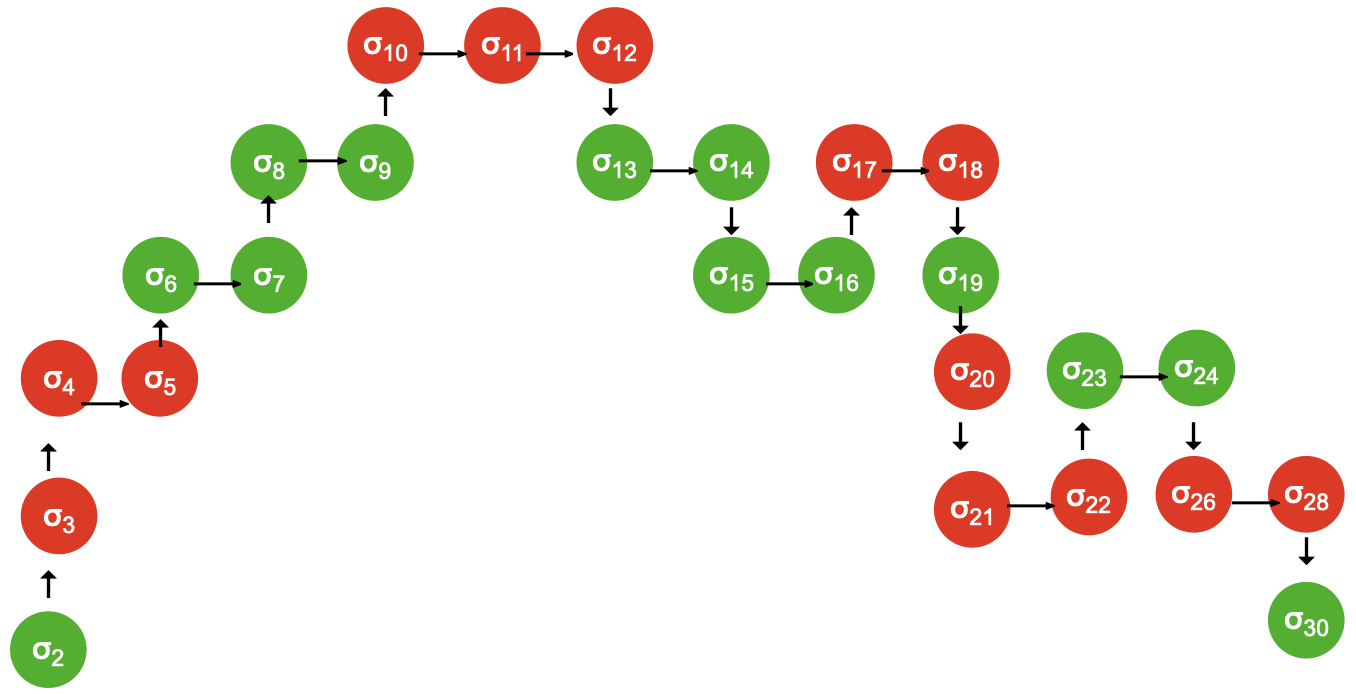
\includegraphics[width=\linewidth]{diagrams/summaryA.png}
} 
\\
\hline \\
the summarised execution:
\\
~ \\
\resizebox{9cm}{!}
{
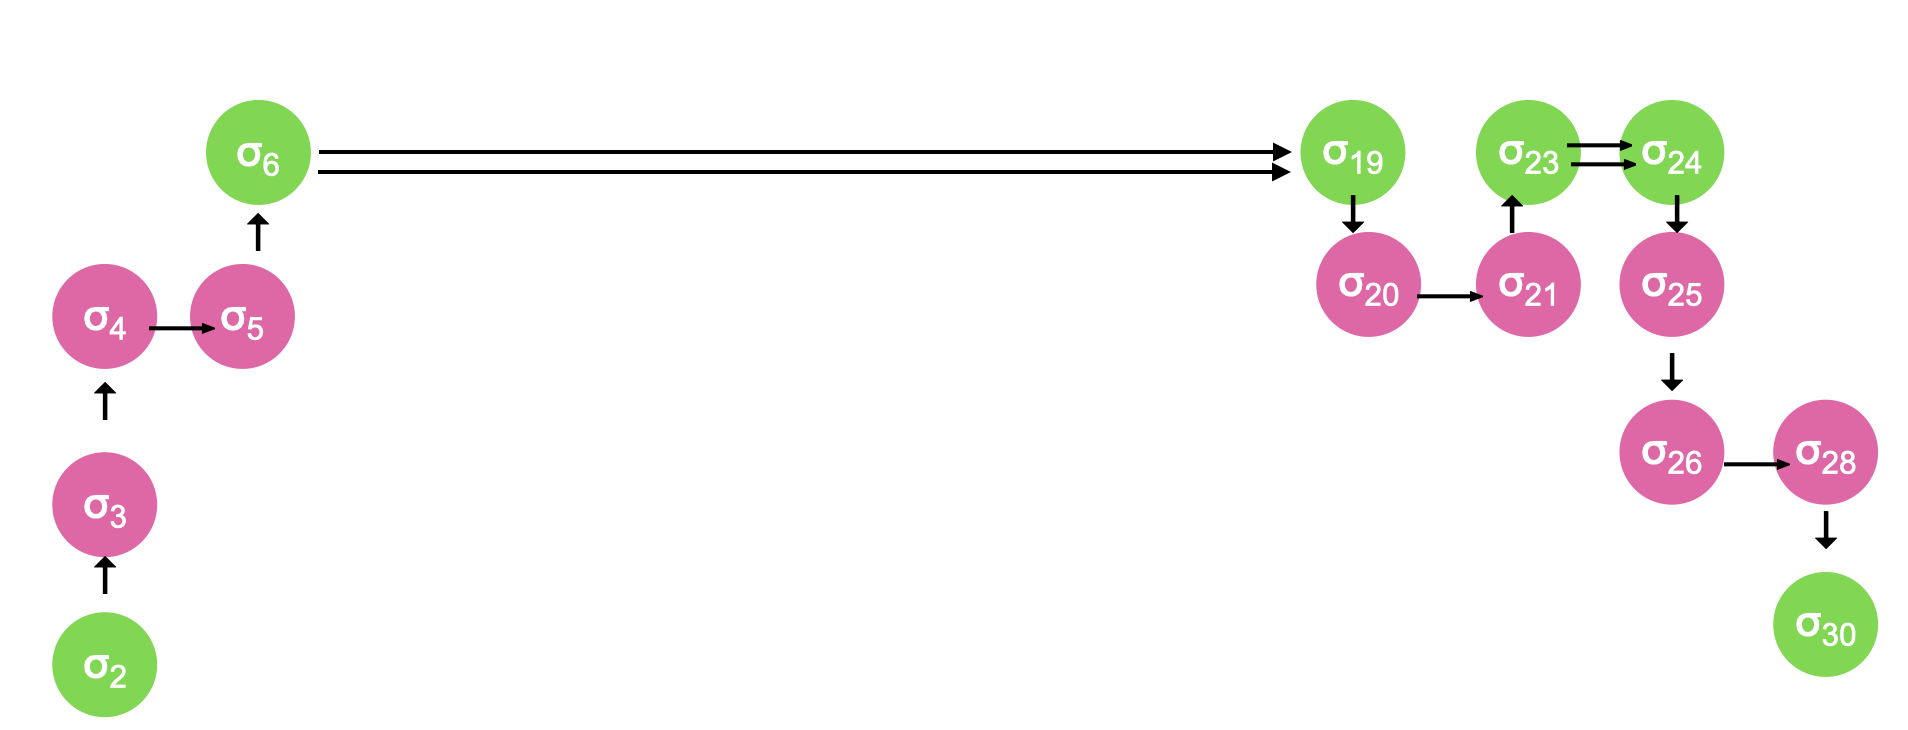
\includegraphics[width=\linewidth]{diagrams/summaryB.png}
} 
\\
\hline \hline
\end{tabular}
   \caption{Summaries. 
   }
   \label{fig:summaries}
 \end{figure}

The lemma \ref{lemma:external_exec_preserves} describes how an encapsulated assertion $A$ is preserved during an execution, provided that all finalizing internal executions preserved it. 
It will be used in the proof of soundness of the rule {\sc{ExtCall\_WithSpec\_Weak}}\footnoteSD{perhaps also {\sc{ExtCall\_WithSpec\_Strong}}}


%\begin{auxLemma}
%\label{lemma:external_exec_preserves}[Preservation of Encapsulated Assertions]
%For any module $M$, modules $\Mtwo$, variables $\overline x$, and addresses $\overline \alpha$,
% states $\sigma\bd$, $\sigma$, and $\sigma'$, and assertions $A$, $A'$:
%
%Assume that $M \models \encaps A \   \wedge  \ A'\txteq A[\overline{\alpha/x}]\  \wedge \ fv(A)=\emptyset \  \wedge \ 
%M, \sigma \models  A' $. Then
%
%\begin{itemize}
%\item
%$   \leadstoBoundedThreeStarExt {\Mtwo\cdot M} {\sigma\bd}  {\sigma}  {\sigma'} 
%\ \ \Longrightarrow \ \ \ M, \sigma' \models A'$
%\item
%$ \leadstoBoundedThreeStarExt {\Mtwo\cdot M} {\sigma\bd}  {\sigma}  {\sigma'} \ \mbox{as a return from a method}
%\ \ \Longrightarrow \ \ \ M, \sigma' \models A'$
%\item
%\end{itemize}
%\end{auxLemma}

 


\begin{auxLemma}
\label{lemma:external_exec_preserves_more}[Preservation of Encapsulated Assertions]
For any module $M$, modules $\Mtwo$, variables $\overline x$, and addresses $\overline \alpha$,
 states $\sigma\bd$, $\sigma$, and $\sigma'$, and assertions $A$, $A'$, 
assume that

\noindent
 $M \models \encaps A \   \wedge  \ A'\txteq A[\overline{\alpha/x}]\  \wedge \ fv(A)=\emptyset \  \wedge \ 
M, \sigma \models  A' $. Then

\begin{enumerate}

\item
$   \leadstoBoundedThreeStarExt {\Mtwo\cdot M} {\sigma\bd}  {\sigma}  {\sigma'} 
\ \ \Longrightarrow \ \ \ M, \sigma' \models A'$

\item
$M, \sigma  \models \extThis \ \wedge \  \leadstoBoundedThree  {\Mtwo\cdot M} {\sigma} {\sigma}  {\sigma_{1}} \ \wedge
 \ M, \sigma_1 \models \pubMeth \ \wedge\  \leadstoBoundedStarFin {\Mtwo\cdot M} {\sigma_1}  {\sigma_2}    \ \ \wedge$\\
$ M, \sigma_2 \models A' \ \wedge \ 
  \   \leadstoBounded  {\Mtwo\cdot M} {\sigma_2}      {\sigma'}$\\
 $\Longrightarrow $
\\
$M, \sigma' \models A' $

\item
$ \WithExtPub {\Mtwo\cdot M} {\sigma\bd}  {\sigma}  {\sigma'} {\sigma_1...\sigma_n}\ \ \wedge $\\
 $\strut \ \ \ \  \  \forall i\in [1..n]. \forall \sigma_{f}.[ \ \  M, \sigma_i \models A'  \ \wedge \  \leadstoBoundedStarFin {M\cdot \Mtwo}  {\sigma_i}  {\sigma_{f}} \ 
\Longrightarrow \  M, \sigma_f \models A' \ ]$\\
$\Longrightarrow $
\\
$M, \sigma' \models A' $
\end{enumerate}

TOTHINK: Do we also need that $A$ is a module invariant?
\end{auxLemma}
%$\strut \ \ \ \  \forall i\in [1..q).[\   \leadstoOrig {M\cdot \Mtwo}  {\sigma_i}  {\sigma_{i+1}}\  ] \  \ \ \wedge$\\
%$\strut \ \ \ \  m_1=1 \ \wedge\ n_p=q+1 \  \wedge\ \forall i\in[1..p).[  \  m_i < n_i < m_{i+1}  ] \ \wedge \ m_p<n_p\ \ \wedge  $\\
%$\strut \ \ \ \  \forall i\in[1..p].\forall j\in [m_i..n_i)[\   M,\sigma_j \models \external {\texttt{this}} \ ] \  \ \ \wedge$\\
%$\strut \ \ \ \ \forall i\in[1..p). [ \ M,\sigma_{n_i} \models A   \ \Rightarrow \ \ 
%M, {\sigma_{m_{i+1}-1}} \models A  \ ] $ \\
%then\\
%$\strut \ \ \ \  \ M, \sigma_q \models  A$
%\end{auxLemma}


% KEEP In case we need
%\begin{auxLemma}
%\label{lemma:external_exec_preserves}[Preservation of Encapsulated Assertions]
%For any module $M$, modules $\Mtwo$, numbers $p$ and $q$, states$\sigma_1$, .... $\sigma_p$,  numbers $m_1,...m_p, n_1, ... n_p \in \mathbb{N}$, and assertions $A$:
%\\
%If \\
%$\strut \ \ \ \  M, \sigma_1 \models  A   \  \ \wedge \ \ M \models \encaps A \ \ \ \  \ \ \wedge$\\
%$\strut \ \ \ \  \forall i\in [1..q).[\   \leadstoOrig {M\cdot \Mtwo}  {\sigma_i}  {\sigma_{i+1}}\  ] \  \ \ \wedge$\\
%$\strut \ \ \ \  m_1=1 \ \wedge\ n_p=q+1 \  \wedge\ \forall i\in[1..p).[  \  m_i < n_i < m_{i+1}  ] \ \wedge \ m_p<n_p\ \ \wedge  $\\
%$\strut \ \ \ \  \forall i\in[1..p].\forall j\in [m_i..n_i)[\   M,\sigma_j \models \external {\texttt{this}} \ ] \  \ \ \wedge$\\
%$\strut \ \ \ \ \forall i\in[1..p). [ \ M,\sigma_{n_i} \models A   \ \Rightarrow \ \ 
%M, {\sigma_{m_{i+1}-1}} \models A  \ ] $ \\
%then\\
%$\strut \ \ \ \  \ M, \sigma_q \models  A$
%\end{auxLemma}



\subsection{A well-founded ordering}
\label{sect:prove:wellfounded}

We will prove soundness by well-founded induction.
% \footnote{This kind of induction is described in \texttt{https://en.wikipedia.org/wiki/Well-founded\_relation.}}
We start by designing a well--founded ordering. 



\sdN{
\begin{definition}
For a module $M$, modules $\Mtwo$, assertions $A_1$, $A_2$, $A_3$, $A_4$, $A_5$,  $A_6$, states $\sigma_1$, $\sigma_2$, and   $P$ a set of proof trees for triples of the form 
$M \vdash \quadruple {A} {stm} {A'} {A''}$,  we define a measure
, $\measure {A, \sigma,A',A''} {M,\Mtwo,P} $, and based on it, a well founded ordering $(A_1,\sigma_1,A_2, A_3) \ll_{M,\Mtwo,P}  (A_4,\sigma_2,A_5,A_6)$
as follows:
\begin{itemize}
\item
 $\measure {A, \sigma,A',A''} {M,\Mtwo,P} $ = $(m, n)$, \ \ \  if\\
$m$ is the minimal number so that $\exists \sigma'.[\ \leadstoBoundedStarFin {M\cdot \Mtwo} {\sigma}    {\sigma'}\ ]$ in $m$ execution steps, \\
 and $n$ is minimal depth of all proofs of $M \vdash \quadruple {A} {\sigma.\prg{cont}} {A'} {A''} $ in $P$,
 \item
 $(m,n) \ll (m',n')$\ \ if \ \ `$(m<m'\vee  (m=m'  \wedge n < n')$.
\item
$(A_1,\sigma_1,A_2, A_3) \ll_{M,\Mtwo,P}  (A_4,\sigma_2,A_5, A_6)$ iff
\\
$\measure {A_1, \sigma_1,A_2, A_3} {M,\Mtwo,P}  \ll \measure {A_4, \sigma_2,A_5. A_6} {M,\Mtwo,P} $
%old def
%\begin{enumerate}
%\item
%$P$ has a proof for $M \vdash \{ A_2 \} \ \sigma_2.\texttt{cont}\  \{ A_4 \} $, and one of the direct predecessors of that proof in $P$ is $M \vdash \{ A_1 \}\ \sigma_1.\texttt{cont}  \{ A_3 \} $ \\
%or
%\item
% $\leadstoBoundedStar {M\cdot \Mtwo} {\sigma_2}    {\sigma_1}$, and $M \vdash \{ A_1 \}\ \sigma_1.\texttt{cont}\  \{ A_3 \} $ is proven in $P$
%\end{enumerate}
\end{itemize}
\end{definition}
}


\begin{auxLemma}
\label{lemma:normal:two}
For any modules $M$,$\Mtwo$,   and  a % normalized  set of proof trees 
$P$, the relation $\_ \ll_{M,\Mtwo,P}  \_$
is well-founded.
\end{auxLemma}

  
  %%%%%%%%%%%%%%%%%%%%%%%%%%%%%%%%%%%%%%%%%%%%%%%%%%%

\subsection{ Soundness of  Hoare Quadruples Logic}
\label{sect:prove:sound:quadruples}
We now prove soundness of the inference system $M \vdash  \quadruple A {stmt} {A'} {A''}$:


\begin{theorem}
For module  $M$ % and $\Mtwo$, 
such that  $\vdash M$, and for any assertions $A$ and $A'$, and statement  $stmt$, we have

\begin{center}
$M\ \vdash\  \quadruple {A} {stmt} {A'} {A''}$ \ \ \ \ implies \ \ \ \ $M\ \models\  \quadruple {A} {stmt} {A'} {A''}$
\end{center}

\end{theorem}

\noindent
\vspace{.2cm}
  {\textbf{Proof Sketch}} 

Take any $M$, $\Mtwo$, $A_{one}$, $A_{two}$, $A_{inv}$ and $stmt$.\\ Assume that $\vdash M$  and 
$M\ \vdash\  \quadruple {A_{one}}  {stmt}{A_{two}} {A_{inv}}$.
% By lemma  \ref{lemma:normal:one}) there exists a set of normalized 
Therefore, there exists a set of
proof trees $P$ which prove  the two judgments from above.
% hat\\ $\vdash M$, \ \  and also prove that \\
% $M\ \vdash\  \quadruple {A_{one}}  {stmt}{A_{two}} {A_{inv}}$.
 
 We have that \\
 $\strut \ \ \hspace{2.3cm} \ \ (1a) \ \ \vdash M $\ \ \  is proven in $P$.\\
$\strut \ \ \hspace{2.3cm} \ \ (1b) \ \ M\ \vdash\  \quadruple {A_{one}}  {stmt}{A_{two}} {A_{inv}}$ \ \  is proven in $P$.
\\
We want to show  that\\
 $\strut \ \ \hspace{2.3cm} \ \ (\alpha)\  \  M\ \models\  \quadruple {A_{one}}  {stmt}{A_{two}} {A_{inv}}$. 
 \\ 
We shall prove,  by induction on $\_ \ll_{M,\Mtwo,P}  \_$, that 
\\ 
$(*) \hspace{1cm} \forall A, A', A'' \sigma, \sigma',\sigma''[$\\
$\strut \ \ \hspace{2.3cm} \ \ (2) \ \ M\ \vdash\  \quadruple {A}  {\sigma.\prg{cont}} {A'} {A''} \ \ $ is proven in $P$,\\
$\strut \ \ \hspace{2.3cm} \ \ (3) \ \ M, \sigma \models A$, \\
$\strut \ \ \hspace{2.3cm} \ \ (4) \ \ \leadstoBoundedStarFin {\Mtwo\cdot M}  {\sigma}  {\sigma'}$,\\
$\strut \ \ \hspace{2.3cm} \ \ (5) \ \ \leadstoBoundedStar  {\Mtwo\cdot M}  {\sigma}  {\sigma''}$,\\
$\strut \ \ \hspace{2.3cm} \ \ \ \ \ \ \ \ \ \Longrightarrow$\\
$\strut  \ \ \hspace{2.3cm} \ \ (\beta)\ \  M, \sigma' \models A'$,\\
$\strut  \ \ \hspace{2.3cm} \ \ (\gamma)\ \  M, \sigma'' \models [\external{this} \rightarrow A'']$.\\
$\strut \ \   \hspace{1cm} ]$
.
\\
Then the  theorem follows by substituting $A_{one}$, $A_{two}$, and $A_{inv}$ for $A$, $A'$, and $A''$ into (*).


\vspace{.1cm}
\noindent
\textbf{Proof of (*)}\\
By lemma \ref{lemma:normal:two} the relation $\_ \ll_{M,\Mtwo,P}  \_$ is well-founded.
\\
Take any $A, A', A'', \sigma, \sigma'$. Assume  (1), (2), (3),  (4), and (5).
Proceed by case analysis on the proof rule applied to obtain last step in $P$'s proof of (2).

\begin{description} 

\item[{\sc{extend}}] 

By soundness of the underlying Hoare logic, we obtain that  $M\ \models\ \triple {A_{one}} {stmt}   {A_{two}}$. Moreover, 
by the assumption of {\sc{extend}}, $stmt$ does not contain any method call. Rest follows by lemma \ref{l:no:call}.

\item[{\sc{inv}}] 

By Theorem \ref{l:triples:sound}.

\item[{\sc{types-2}}] 

...

\item[{\sc{combine}}] 
 ...

\item[{\sc{sequ}}] 
Therefore, there exist statements $s_1$ and $s_2$, and assertions  $A_1$, $A_2$ and $A''$, so that $A_1\txteq A$, and $A_2 \txteq A'$, and $\sigma.\prg{cont}\txteq  s1; s2$, and
the proof of  $(2)$ %$M\ \vdash\  \{\, A \,  \}\ s_1;s_2\  \{\, A' \, \}$ in $P$ 
has as its immediate predecessors proofs for 
$M\ \vdash\  \quadruple {A_1} {s_1} {A_2} {A''}$ and $ M\ \vdash\  \quadruple {A_2} {s_2} {A_3} {A''}$.

Define $\sigma_1$ as  $\sigma_1 \triangleq \sigma[\prg{cont} \mapsto s_1]$.
Therefore,  $(A_1,\sigma_1,A_2, A'') \ll_{M,\Mtwo,P} (A_1,\sigma,A_3, A'')$. 

By lemma \ref{lemma:subexp} we obtain that there exists a $\sigma_3$ such that $\leadstoBoundedStarFin {\Mtwo\cdot M}  {\sigma_1}  {\sigma_3'}$. 
 By application of the induction hypothesis we obtain that $M, \sigma_3  \models A_3$. 
 
 Define $\sigma_2$ as  $\sigma_2 \triangleq \sigma_3[\prg{cont} \mapsto s_2]$
Therefore, we have that $(A_2,\sigma_2,A_3,A'') \ll_{M,\Mtwo,P} (A_1,\sigma,A_3, A'')$. 

 
Again by lemma \ref{lemma:subexp}, we obtain that $\leadstoBoundedStarFin {\Mtwo\cdot M}  {\sigma_2}  {\sigma'}$.  
 By application of the induction hypothesis we obtain that $(\beta)$, ie that \ \ $ M, \sigma' \models A'$.
 
Let us now take an arbitrary $\sigma''$ such that   $\leadstoBoundedStar  {\Mtwo\cdot M}  {\sigma}  {\sigma''}$. By
lemma  \ref{lemma:subexp}, either $\leadstoBoundedStar  {\Mtwo\cdot M}  {\sigma_1}  {\sigma''}$ or
$\leadstoBoundedStar  {\Mtwo\cdot M}  {\sigma_2}  {\sigma''}$. In the first case, $\leadstoBoundedStar  {\Mtwo\cdot M}  {\sigma_1}  {\sigma''}$. Then, because $(A_1,\sigma_1,A_2, A'') \ll_{M,\Mtwo,P} (A_1,\sigma,A_3, A'')$, we can apply the inductive hypothesis, and obtain $(\gamma)$, ie that \ \ $ M, \sigma'' \models A''$. The second case is analogous.

\item[{\sc{consequ}}] Similar to the proof of  {\sc{combine}}. 


\item[ {\sc{Call\_A}}]

Therefore, there exist $u$, $y_o$, $C$, $\overline y$,  $A_1$ and $A_2$ such that \\
%\begin{tabbing}
(6)\ $\sigma.\prg{cont}\txteq u=y_0.m(\overline y)$,   \hspace{2cm}
 (7)\ $A \txteq y_0:C  \ \wedge\ \overline {y:C}\ \wedge \  A_1$, 
\\ 
 (8)\ $\promises  M {\mprepostN {A_1}{C}{m}{y}{C}{A_2} {A''}}$,    \hspace{1cm}
 (9)\ $A' \txteq  A_2[ u/result]$. 
% \end{tabbing}

By (1), (8), and definition of $\vdash M$ in Section \ref{sect:wf}, we obtain that   $\prg{mBody}(m,C,M)=\overline{y:C}\{\  s \ \}$ and that\\
(10) \  $M \vdash  \quadruple { \ \prg{this}:\prg{C}\, \wedge\, \overline{y:C}\, \wedge\, A_1\  } {\ s\ } {\ A_2\ } {A''}$ is proven in $P$.
 
 By the operational semantics, we obtain that there exist states $\sigma_1$, and $\sigma_2$, such that \\
 (11)\ $\sigma_1=\sigma.PUSHFRAME(\prg{this}, {\overline y} \mapsto \overline{\interpret {\sigma} y},\prg{cont} \mapsto s) $, TODO   \hspace{1cm}
   (12)\ $\leadstoBounded  {\Mtwo\cdot M}  {\sigma}  {\sigma_1}$ \\
 (13)\ $\leadstoBoundedStarFin {\Mtwo\cdot M}  {\sigma_1}  {\sigma_2}$,   \hspace{3cm}
 (14)\ $\sigma'=\sigma_2[...]$ TODO.
 
 From (3), (11) and lemma \ref{lemma:push}.\ref{pushOne}  we obtain that \ \ \  $ (15) \ \ M, \sigma_1 \models \overline{y:C}\, \wedge\, A_1$.\footnote{\red{Here some renaming needed,  but easy to do0.}}
 
 From (10), (11) and (12) we obtain that $( \prg{this}:\prg{C}\, \wedge\, \overline{y:C}\, \wedge\, A_1,\sigma_1,A_2) \ll_{M,\Mtwo,P} (A,\sigma,A')$. By induction hypothesis, (15) and (13) we obtain that (16) $M,\sigma_2 \models A_2$.
 
 By (14) and lemma  \ref{lemma:push}.\ref{pushTwo}  we obtain that 
\ \ $M,\sigma' \models \PushAS  {y} {A_2[ u/result]}$. \. With (9) this gives $M,\sigma' \models A'$.

\item[ {\sc{Call\_B}}]

Therefore, there exist $u$, $y_o$, $C$, $\overline y$,  $A_1$ and $A_2$ such that \\
%\begin{tabbing}
6)\ $\sigma.\prg{cont}\txteq u=y_0.m(\overline y)$,   \hspace{2cm}
 (7)\ $A \txteq y_0:C  \ \wedge\ \overline {y:C}\ \wedge \  (\PushAS  {y} {A_1})$, 
\\
 (8)\ $\promises M {\mprepost{A_1}{C}{m}{y}{C}{  {A_2}} }$,    \hspace{1cm}
 (9)\ $A' \txteq  {\PushAS  {y} {(A_2[ u/result])}}$. 
% \end{tabbing}

By (1), (8), and definition of $\vdash M$ in Section \ref{sect:wf}, we obtain that   $\prg{mBody}(m,C,M)=\overline{y:C}\{\  s \ \}$ and that\\
(10)   ${\hproves{M} { \ \prg{this}:\prg{C}\, \wedge\, \overline{y:C}\, \wedge\, A_1\  } {\ s\ } {\ A_2\ } }$ is proven in $P$.
 
 By the operational semantics, we obtain that there exist states $\sigma_1$, and $\sigma_2$, such that \\
 (11)\ $\sigma_1=\sigma.PUSHFRAME(\prg{this}, {\overline y} \mapsto \overline{\interpret {\sigma} y},\prg{cont} \mapsto s) $, TODO   \hspace{1cm}
   (12)\ $\leadstoBounded  {\Mtwo\cdot M}  {\sigma}  {\sigma_1}$ \\
 (13)\ $\leadstoBoundedStarFin {\Mtwo\cdot M}  {\sigma_1}  {\sigma_2}$,   \hspace{3cm}
 (14)\ $\sigma'=\sigma_2[...]$ TODO.
 
 From (3), (11) and lemma \ref{lemma:push}.\ref{pushOne}  we obtain that \ \ \  $ (15) \ \ M, \sigma_1 \models \overline{y:C}\, \wedge\, A_1$.\footnote{\red{Here some renaming needed,  but easy to do0.}}
 
 From (10), (11) and (12) we obtain that $( \prg{this}:\prg{C}\, \wedge\, \overline{y:C}\, \wedge\, A_1,\sigma_1,A_2) \ll_{M,\Mtwo,P} (A,\sigma,A')$. By induction hypothesis, (15) and (13) we obtain that (16) $M,\sigma_2 \models A_2$.
 
 By (14) and lemma  \ref{lemma:push}.\ref{pushTwo}  we obtain that 
\ \ $M,\sigma' \models \PushAS  {y} {A_2[ u/result]}$. \. With (9) this gives $M,\sigma' \models A'$.

\item[${\sc{ExtCall\_WithSpec\_Weak}}$]

Therefore, there exist $u$, $y_o$, $C$, $\overline y$,  $A_1$ and $A_2$ such that \\
(6)\ $\sigma.\prg{cont}\txteq u=y_o.m(\overline y)$,  \hspace{2cm}
 (7)\ $A \txteq   { \external{y_0} }\, \wedge \, \overline {x:C}  \, \wedge \,  \red{\PushAS  {y}{  A_1} \,   \wedge \,  \PushAS {y}{\extract{M}}}\ $,\footnote{\red{There is a relation between $A_1$ and  $\extract{M}$ -- we should revisit that. 
 But the proof structure is unaffected.}}
\\
 (8)\ $\promises M   {\TwoStatesQ {\overline {x:C}} {A_1}{A_2}}$ \ \ proven in $P$,   \hspace{1cm}
 (9)\ $A' \txteq \PushAS  {y} { A_2}$. 
 \\
 %By (8) and (1), and axiom \ref{lemma:axiom:enc:assert}, we obtain \ \ \ (10) \ $M \models \encaps{A}$.
% \\
 By the operational semantics, we obtain that there exist states $\sigma_{e\_1}$, and $\sigma_{e\_1}$, such that \\
 (11)\ $\sigma_{e\_1}=\sigma ...[\prg{cont}\mapsto s]... $, TODO   \hspace{1cm}
   (12)\ $\leadstoBounded  {\Mtwo\cdot M}  {\sigma}  {\sigma_{e\_1}}$ \\
 (13)\ $\leadstoBoundedStarFin {\Mtwo\cdot M}  {\sigma_{e\_1}}  {\sigma_{e\_2}}$,   \hspace{1cm}
 (14)\ $\sigma'=\sigma_{e\_1}[...]$ TODO.
\\
By (8) and (2) we obtain that there exists an $A_0$ \\
(15)\ $\TwoStatesQ {\overline {x:C}} {A_0}{A_0} \in HS(M)$\\ and \\
 (16) $M \vdash A_1 \rightarrow A_0$ proven in $P$ \ \ \ \ \ \ \  (17) $M \vdash A_0 \rightarrow A_2$ proven in $P$ \\
By (7) and (3) we obtain \ \ 
(18) $M, \sigma \models \extThis$, %\hspace{2cm) 
\\
By (3), (7), (11), (16) and lemma  \ref{lemma:push}.\ref{pushOne} , we get \ \ \ \  (19) $M, \sigma_{e\_1} \models  {  A_0} \,   \wedge \,  {\extract{M}} \, \wedge \, 
\overline{ {\interpret \sigma x} : C}$.
\\
By (8) and (1), and axiom \ref{lemma:axiom:enc:assert}, we obtain \ \ \ (20) \ $M \models \encaps{{  A_0} \,   \wedge \,  {\extract{M}} \, \wedge \, 
\overline{ {\interpret \sigma x} : C}}$.
\\
By (4) and (18), we can apply auxiliary lemma 
\ref{lemma:external_breakdown} and break down the execution from $\sigma_{e\_1}$ to  $\sigma_{e\_2}$ into the internal and external executions as follows:
%For any module $M$, modules $\Mtwo$, states $\sigma$ and $\sigma'$:
\\
There exists $ p,q\in \mathbb{N},  \sigma_1, ... \sigma_q \in States, m_1,...m_p, n_1, ... n_p \in \mathbb{N}.$, such that \\ 
% $\strut \ \ \ \ \ \ \ \ \ \ [  $ \\
$\ \strut \ \ (21) \ \sigma_1=\sigma_{e\_1} \ \ \wedge\ \  \sigma_p=\sigma_{e\_2}\ \  \wedge\ \ \forall i\in [1..q).[\   \leadstoOrig {M\cdot \Mtwo}  {\sigma_i}  {\sigma_{i+1}}\  ] \  \ \ \wedge$\\
$\ \strut \ \ (22) \ \ m_1=1 \ \wedge\ n_p=q+1 \  \wedge\ \forall i\in[1..p).[  \  m_i < n_i < m_{i+1}  ] \ \wedge \ m_p<n_p\ \ \wedge  $\\
$\ \strut \ \ (23) \ \ \forall i\in[1..p].\forall j\in [m_i..n_i)[\   M,\sigma_j \models \external {\texttt{this}} \ ] \  \ \ \wedge$\\
$\ \strut \ \ (24) \ \ \forall i\in[1..p). [ \ M,\sigma_{n_i} \models \internal {\texttt{this}}   \ \wedge \ \ 
 \leadstoBoundedStarFin {M\cdot \Mtwo}  {\sigma_{n_{i}}}  {\sigma_{m_{i+1}-1}} \ ] $ \\
%$\strut \ \ \ \ \ \ \ \ \ \ ]$
From (12), and (21) we obtain that\\
$\ \strut \ \ (25)\   \forall i\in[1..p). [ \ \leadstoBoundedStar {M\cdot \Mtwo}  {\sigma} {\sigma_{n_{i}}} \ ]$\footnote{needs so tidying up, but easy}
\\
From  (24) and (15) and (1) we obtain that\\
$\ \strut \ \ (26)\ \forall i\in[1..p). [ \ M\vdash \{ \, A_0  \}\, {\sigma_{n_{i}}.\prg{cont}}  \{ \, A_0 \}\ \  \mbox{ is proven in } P \ ]$\footnote{\red{because of the design issue it could be that we would have $\extract M$ rather than $A_0$ -- but this is an orthogonal dewsign question, and the soundness argument would hold either way.}}, \\
\\
From (25) and (26) we obtain that\\
$\ \strut \ \ (27)\   \forall i\in[1..p).[ \ ( A_0, \sigma_{n_{i}}, A_0 ) \ll_{M,\Mtwo,P}  A, \sigma, A' )\ ]$
\\
From (24), (26), (27), and the induction hypothesis, we obtain\\
$\ \strut \ \ (28)\    \forall i\in[1..p).[ \ \  M, \sigma_{n_{i}} \models A_0 \ \Longrightarrow \ \ M, \sigma_{m_{i+1}-1} \models A_0 \ \ ]$.\\
We apply auxiliary lemma \ref{lemma:external_exec_preserves} on (19), (20) (21), (22), (23), (28), and obtain\\
$\ \strut \ \ (29) \   M, \sigma_{e\_2} \models A_0$.\\
We now apply lemma \ref{lemma:push}.\ref{pushTwo} on (29) and  (14) and obtain\\
$\ \strut \ \ (30) \   M, \sigma'  \models \PushAS  {y}{A_0}$.
We apply (17) on (30) and obtain\\
$\ \strut \ \ (30) \   M, \sigma'  \models \PushAS  {y}{A_2}$.
\end{description}
\noindent
\vspace{.1cm}
  {\textbf{End Proof Sketch}} 

\vspace{1cm}

  %%%%%%%%%%%%%%%%%%%%%%%%%%%%%%%%%%%%%%%%%%%%%%%%%%%
  \subsection{Soundness of the overall system}
\label{sect:prove:triples:overall}
Finally, we can now prove soundness of the overall system

\begin{theorem}[Soundness]
\label{thm:soundness}
Assume an \SpecO proof system, $\proves{M}{A}$, 
an encapsulation inference system, $\proves{M}{\encaps{A}}$,
% Axiom xx, and 
 and  that on top of these systems we built
 the \SpecLang logic according to zzzz,  then, for    all modules $M$, and all \SpecLang specifications  $S$:
 
 $$\proves{M}{S}\ \ \ \ \ \ \ \mbox{implies}\ \ \ \ \ \  \ \ \ \satisfies{M}{S}$$
\end{theorem}

\begin{proof}
% follows from earlier theorem and the axiom.
TODO: We will make a similar argument as for method calls in previous subsection, and will be using AuxLemma 8.4
% by induction on the derivation of $\proves{M}{S}$.
\end{proof}
 


Theorem. \ref{thm:soundness} demonstrates 
 that the   \SpecLang logic is sound with respect to the semantics of \SpecLang specifications.
 The \SpecLang logic parametric wrt to the algorithms for proving validity of assertions
 $\proves{M}{A}$, and 
 assertion encapsulation ($\proves{M}{\encaps{A}}$), and is sound
 provided that these two proof systems are sound.